\documentclass[11pt]{article}
\usepackage[T1]{fontenc}
\usepackage[margin=1in]{geometry}
\usepackage{amsmath,amssymb,amsthm}
\usepackage{booktabs}
\usepackage{graphicx}
\graphicspath{{figures/}}
\usepackage{microtype}
\usepackage{hyperref}
\usepackage{enumitem}
\usepackage{placeins}
\usepackage{siunitx}
\usepackage{xcolor}
\hypersetup{colorlinks=true,linkcolor=blue,citecolor=blue,urlcolor=blue}
\newtheorem{theorem}{Theorem}
\newtheorem{lemma}{Lemma}
\newtheorem{proposition}{Proposition}
\newcommand{\depot}{\delta}
\newcommand{\OPT}{\mathrm{OPT}}
\title{Capacity-Aware Completion Bounds for Exact Fixed-Permutation Electric Vehicle Routing Decoding}
\author{Ryutaro Yonezu\\Independent Researcher}
\date{September 5, 2026\\Preprint candidate -- not peer reviewed}

\begin{document}
\maketitle

\begin{abstract}
The recently introduced Fixed-Permutation Splitting and Charging Problem (FPSCP) asks for a minimum-distance feasible electric-vehicle routing solution obtained by inserting depot returns and charging-station visits into a fixed customer permutation. Its exact forward-labeling algorithm, FP-FLA, provides an optimal decoding but repeatedly expands non-dominated labels through pairs of energy-reset nodes. This paper develops an admissible capacity-aware completion bound that can reject a label before those pair expansions. The bound solves a relaxation that preserves the remaining customer order and residual cargo capacity while dropping battery constraints. A suffix split dynamic program and a range-minimum structure make the bound depend only on the FP-FLA stage and current cargo resource, so no hidden history is added to the label state and the original dominance rule remains valid.

A source-matched C++ implementation was evaluated on six public WCCI-2020 EVRP instances. For each instance, 20 nearest-neighbor-biased and 20 random customer permutations were tested, for 240 public cases in total. Every bounded run returned the same objective value as an unbounded, source-matched FP-FLA reference that retained the original feasibility and Pareto-dominance pruning but used no incumbent or completion-bound pruning. Relative to incumbent-bounded FP-FLA using the same feasible incumbent, the capacity-aware variant achieved a median preprocessing-inclusive decoder speedup of \textbf{14.41x} (bootstrap 95\% CI 12.62--16.00x), while removing a median \textbf{73.2\%} of charging-station pair enumerations. The initial incumbent was strictly worse than the source-matched reference objective in 131 of 240 public cases. A further 996 feasible synthetic stress cases produced no objective mismatch against the same reference construction; 425 of these used a strictly nonoptimal initial incumbent.

As an additional implementation check, a separate direct-upstream gate compiled the pinned public FPSCP core at commit \texttt{db9ccca30f2def5fabf85e65958d52dcae0cefd6} and compared upstream \texttt{OptimalDecode} with a lazy split-DAG wrapper whose expensive block oracle was the upstream \texttt{BatteryDecode}. Across 17 public EVRP instances, 10 random and 10 nearest-neighbor-biased permutations per instance yielded \textbf{340/340} objective matches; \textbf{34/34} independently selected clean-room checks also matched. This direct-upstream gate is an exactness/compatibility check, not the same timing experiment as the 14.41x capacity-bound benchmark and not an independent MIP/CP certificate. These results support a narrow conclusion: completion bounding is not new to labeling algorithms, but a cargo-aware specialization to FPSCP can materially accelerate the exact joint split-and-charge decoder while preserving its optimum value.
\end{abstract}

\section{Introduction}
Permutation representations are common in routing metaheuristics, but an electric-vehicle routing permutation is not itself a feasible routing solution. Depot returns must be inserted to satisfy cargo capacity, and charging-station visits must be inserted to satisfy the battery constraint. These decisions are coupled because a depot visit both separates routes and resets energy. Uroi\'c and \DJ urasevi\'c formalized this decoding task as the Fixed-Permutation Splitting and Charging Problem (FPSCP) and introduced FP-FLA, an exact forward-labeling algorithm that finds a minimum-distance feasible decoding of a fixed customer permutation \cite{uroic2026}.

The value of an exact decoder is clear: it gives the optimal value for a fixed permutation and therefore provides a reference against which restricted or heuristic decoders can be measured. The cost is that FP-FLA extends every surviving label by direct travel and by nested pairs of reset nodes (charging stations plus the depot), after which dominance pruning collapses the generated labels. The parent work explicitly reports a quality--runtime hierarchy: increasingly restricted decoders run faster, while the exact joint decoder supplies the optimal reference \cite{uroic2026}.

This paper asks a narrower algorithmic question: \emph{can exact FP-FLA reject a partial label before enumerating its reset-node pairs, using information already implicit in the fixed customer permutation?} The answer is yes. The fixed order allows a capacity-only suffix relaxation to be solved independently of battery decisions. Its optimum is an admissible lower bound on the remaining travel distance. Because the relaxation retains only the current cargo resource and the stage index, the bound does not enlarge the state needed by the original dominance rule.

Completion bounds and lower-bound pruning are classical ideas in constrained shortest-path and vehicle-routing labeling. They have also been used in fixed-route EV charging, including backward time/energy bounds in Froger et al. \cite{froger2019}, and more recent EVRP pricing algorithms explicitly develop completion bounds for charging-aware labeling \cite{enerback2024}. Accordingly, the contribution here is deliberately narrow: a state-compatible, cargo-aware completion bound specialized to the newly formalized FPSCP/FP-FLA setting, together with an exactness proof and a source-matched computational evaluation.

\paragraph{Contributions.} The paper provides:
\begin{enumerate}[leftmargin=*]
    \item a capacity-relaxed completion bound for a partial FP-FLA label;
    \item an $O(n^2)$ per-permutation preprocessing scheme with $O(\log n)$ residual-capacity endpoint lookup and $O(1)$ range-minimum completion queries;
    \item a proof that incumbent pruning with this bound preserves the optimal FPSCP objective value and requires no history variable beyond the original stage and cargo resource;
    \item experiments on 240 public benchmark/permutation cases plus 996 feasible synthetic stress cases, including a fair comparison to FP-FLA using the same incumbent and timing that includes bound preprocessing, together with a separate 340-case direct-upstream compatibility gate against the pinned compiled FPSCP core.
\end{enumerate}

\section{Background and Related Work}
\subsection{FPSCP and FP-FLA}
Let $G=(V,E)$ be a complete metric graph with depot $\depot$, customer set $V_c$, and charging-station set $V_f$. Customer $i$ has demand $q_i$, vehicle cargo capacity is $Q$, battery capacity is $B$, and travel consumes energy proportional to distance. The input is a fixed permutation
\[
\pi=(\pi_1,\ldots,\pi_n).
\]
A feasible decoding inserts depot and charging-station visits while preserving the relative customer order. The objective is total travel distance \cite{uroic2026}.

FP-FLA processes the permutation left to right. At stage $i$, a label contains accumulated distance $d$, battery consumption since the most recent energy reset $b$, and cargo consumed on the current route $q$. A label is extended directly, through charging-station/reset-node paths, or through a depot detour that resets cargo. Non-dominated labels are retained. In the public reference implementation, the reset-node pair loops are nested inside the extension of every surviving label; the decoder also accepts an external upper bound on solution distance.

\subsection{Bounding in EV routing labels}
Lower bounds are not new in EV labeling. Froger et al. use backward Dijkstra computations to obtain lower bounds that accelerate exact fixed-route charging decisions \cite{froger2019}. Kullman et al. provide an open-source exact FRVCP solver, facilitating adoption of such fixed-route charging methods \cite{kullman2021}. Enerb\"ack et al. develop completion bounds for an EVRPTW pricing labeling algorithm and show that problem-specific bounds can substantially reduce labeling effort \cite{enerback2024}. The present method differs in problem structure: FPSCP simultaneously decides route splits and charging insertions from a fixed customer permutation. Our bound exploits the cargo-splitting structure of that permutation and is designed to remain compatible with FP-FLA's original label state.

\section{Capacity-Aware Completion Bound}
\subsection{Notation}
Write $d(u,v)$ for metric distance. Define demand prefixes
\[
P_j=\sum_{r=1}^{j} q_{\pi_r},\qquad P_0=0,
\]
and direct-chain prefixes
\[
C_1=0,\qquad C_j=\sum_{r=1}^{j-1} d(\pi_r,\pi_{r+1})\quad (j\ge 2).
\]
For $i\le j$, the distance of the direct depot-to-depot segment serving consecutive customers $\pi_i,\ldots,\pi_j$ is
\[
D(i,j)=d(\depot,\pi_i)+(C_j-C_i)+d(\pi_j,\depot).
\]

Let $S_i$ be the optimum of the \emph{capacity-only} split problem for suffix $\pi_i,\ldots,\pi_n$, with battery constraints removed:
\begin{equation}
S_i=\min_{j\ge i:\,P_j-P_{i-1}\le Q}\{D(i,j)+S_{j+1}\},\qquad S_{n+1}=0.
\label{eq:suffixdp}
\end{equation}
This dynamic program is $O(n^2)$ in the direct implementation used here.

\subsection{Completion from a partial label}
Consider a label after customer $\pi_i$ has been served, with current cargo resource $q$. It has $Q-q$ residual cargo capacity on the current route. Let
\[
J(i,q)=\max\{j\ge i+1:P_j-P_i\le Q-q\},
\]
when such a $j$ exists. A relaxed completion can either close the current route immediately or append customers through some $\pi_j$ that fits the residual cargo capacity and then close the route. Therefore define
\begin{align}
h_i(q)=\min\Bigg\{&d(\pi_i,\depot)+S_{i+1},\\
&\min_{j=i+1,\ldots,J(i,q)}\big[(C_j-C_i)+d(\pi_j,\depot)+S_{j+1}\big]\Bigg\}.
\label{eq:h}
\end{align}
If no next customer fits, only the close-now term is available. Before the first customer, define $h_0(0)=S_1$.

For fast queries, precompute
\[
A_j=C_j+d(\pi_j,\depot)+S_{j+1}.
\]
Then the inner minimum in \eqref{eq:h} is
\[
\min_{j=i+1}^{J(i,q)} A_j-C_i.
\]
A sparse table gives the range minimum in $O(1)$ after $O(n\log n)$ construction, while $J(i,q)$ is obtained by binary search in the demand-prefix array in $O(\log n)$. The suffix dynamic program remains the dominant $O(n^2)$ preprocessing term.

\begin{lemma}[Admissibility]
For any feasible FP-FLA label at stage $i$ with current cargo $q$, $h_i(q)$ is no larger than the additional distance of any feasible FPSCP completion of that label.
\end{lemma}
\begin{proof}
Take any feasible FPSCP completion. Preserve its customer order and explicit depot returns, but remove every charging-station visit and drop the battery constraint. By the triangle inequality, replacing each station detour by direct travel between its adjacent mandatory nodes cannot increase distance. Dropping the battery constraint can only enlarge the feasible set. The current route may serve only a consecutive prefix of the remaining permutation whose total demand fits $Q-q$; after the next depot return, all later routes form a feasible solution of the capacity-only suffix split problem. Equation \eqref{eq:h} minimizes over exactly this relaxation, so its value cannot exceed the completion's additional distance.
\end{proof}

\begin{theorem}[Safe incumbent pruning]
Let $U$ be the cost of any feasible complete decoding retained as an incumbent. A label with accumulated cost $d$ may be discarded whenever
\[
d+h_i(q)\ge U.
\]
Doing so preserves the optimal FPSCP objective value.
\end{theorem}
\begin{proof}
By admissibility, every feasible extension of the label has total cost at least $d+h_i(q)$. If this is at least $U$, no extension can improve the retained feasible incumbent. If equality holds at the optimum, returning the retained incumbent still preserves the optimum objective value. For solution reconstruction, the incumbent route itself is stored separately.
\end{proof}

\begin{proposition}[Compatibility with FP-FLA dominance]
The bound requires no additional history state beyond the FP-FLA stage and current cargo resource.
\end{proposition}
\begin{proof}
At a fixed stage $i$, $h_i(q)$ is a function only of $q$ and precomputed permutation data. It does not depend on the route start, predecessor identity, or charging history. Thus bound evaluation can be applied to labels after the original FP-FLA dominance rule without modifying the dominance state. Moreover, lower cargo can only weakly increase residual capacity and hence cannot worsen the relaxed completion optimum.
\end{proof}

\section{Implementation}
The implementation follows the public FP-FLA transition structure: direct extension, a charging detour over all ordered pairs of reset nodes (charging stations plus depot), and an explicit depot detour. Reset-node shortest paths are precomputed with Floyd--Warshall under the battery-feasible edge relation, as in the reference implementation. The key change is a parent-level test
\[
d+h_i(q)\ge U
\]
placed before the nested reset-node pair loops. The same bound is also checked on generated candidates before they enter the next Pareto front.

The public FP-FLA interface already accepts an upper bound. To avoid crediting our method for a better incumbent, the principal runtime comparison uses the \emph{same feasible incumbent $U$} for both the incumbent-bounded FP-FLA control and the capacity-aware variant. In the benchmark harness, $U$ is constructed independently by solving the cargo-only split problem and then exactly inserting charging visits on each fixed route segment. If this construction fails, the proposed algorithm may simply use $U=\infty$ until some external feasible incumbent is available; exactness does not depend on a finite initial bound. In all 240 public cases and all 996 feasible stress cases reported below, this construction produced a finite incumbent.

The source-matched implementation was checked against the public FPSCP repository at main commit \texttt{db9ccca30f2def5fabf85e65958d52dcae0cefd6}; the reference \texttt{optimal\_decode.cpp} blob used for structural matching had SHA \texttt{1dd493bcf1410fbb2f626be4a0a06514d9a6d3de}. The artifact bundle accompanying this preprint contains the complete standalone benchmark code, stress code, raw CSV data, analysis script, and preprocessing microbenchmark.

\section{Experiments}
\subsection{Public benchmark protocol}
We used six instances from the public benchmark suite of Mavrovouniotis et al. \cite{mavrovouniotis2020}: E-n29-k4-s7, E-n30-k3-s7, E-n35-k3-s5, E-n37-k4-s4, E-n60-k5-s9, and F-n49-k4-s4. For each instance we generated 20 nearest-neighbor-biased permutations (each next customer sampled from the three nearest remaining customers) and 20 random permutations, yielding 240 cases.

Four exact configurations were evaluated: (i) an unbounded, source-matched FP-FLA reference that retains the original feasibility checks and Pareto-dominance pruning but uses neither incumbent pruning nor a completion bound; (ii) incumbent-bounded FP-FLA, using the feasible $U$ but no completion bound; (iii) a weaker direct-chain lower bound; and (iv) the capacity-aware bound. The unbounded configuration is an internal differential reference, not a brute-force enumeration with all FP-FLA pruning disabled and not an independent MIP/CP oracle. Every bounded configuration was required to match the source-matched reference objective within $10^{-6}$; the program terminates immediately on a mismatch. For each case and decoder configuration, three timed solves were interleaved in randomized order and the median solve time was retained. Bound-specific preprocessing was measured separately over repeated executions and is added to the capacity-aware time in the main speedup calculation.

Measurements were made in a Linux container on an Intel Xeon E5-2673 v4 at 2.30 GHz, using g++ 14.2.0, C++20, and \texttt{-O3}. The absolute microsecond timings are platform-specific; the machine-independent station-pair counts and Pareto-front sizes are therefore reported alongside speedups.

\subsection{Public benchmark results}
All 240 public cases matched the unbounded source-matched reference objective. The initial incumbent was strictly worse than that reference objective in 131/240 cases, so the pruning result is not restricted to cases in which the reference value was supplied as the initial bound. This 240/240 agreement is a differential implementation check; optimality preservation itself follows from Theorem 1, while common-mode errors in the source-matched implementation are not independently excluded by these experiments.

Across all 240 cases, the median speedup of the capacity-aware decoder relative to incumbent-bounded FP-FLA was 14.41x after adding bound preprocessing; a 10,000-resample nonparametric bootstrap gave a 95\% confidence interval of 12.62--16.00x for the median. The median bound preprocessing cost was 1.57 microseconds. The capacity-aware method removed 73.2\% of reset-node pair enumerations and reduced the maximum front size by a median of 74.0\%.

\begin{table}[t]
\centering
\small
\caption{Public benchmark results. Speedup is against incumbent-bounded FP-FLA using the same $U$ and includes capacity-bound preprocessing. Pair reduction is relative to the same incumbent-bounded control. Values are medians over 20 permutations per row.}
\label{tab:public}
\begin{tabular}{llrrrrr}
\toprule
Instance & Perm. & $t_U$ (ms) & $t_{cap}$ (ms) & Speedup & Pair red. & Nonopt. $U$\\
\midrule
E-n29-k4-s7 & knn3   & 1.454 & 0.087 & 17.47 & 78.7\% & 4/20\\
             & random & 0.926 & 0.105 &  9.67 & 65.5\% & 15/20\\
E-n30-k3-s7 & knn3   & 2.172 & 0.100 & 21.09 & 76.9\% & 6/20\\
             & random & 1.250 & 0.158 &  7.64 & 57.4\% & 17/20\\
E-n35-k3-s5 & knn3   & 2.054 & 0.086 & 22.42 & 84.8\% & 13/20\\
             & random & 0.829 & 0.353 &  2.59 & 27.6\% & 20/20\\
E-n37-k4-s4 & knn3   & 1.792 & 0.052 & 35.15 & 91.8\% & 1/20\\
             & random & 1.108 & 0.065 & 16.47 & 84.8\% & 1/20\\
E-n60-k5-s9 & knn3   &12.690 & 0.726 & 18.49 & 73.9\% & 10/20\\
             & random & 5.951 & 0.983 &  5.61 & 45.7\% & 19/20\\
F-n49-k4-s4 & knn3   & 2.623 & 0.102 & 24.43 & 86.2\% & 5/20\\
             & random & 0.990 & 0.247 &  4.42 & 43.6\% & 20/20\\
\bottomrule
\end{tabular}
\end{table}

Figure \ref{fig:speed} shows the effect across all twelve groups, with workload-dependent magnitude. Nearest-neighbor-biased permutations had a median preprocessing-inclusive speedup of 21.51x, while random permutations had a median of 6.42x. This is consistent with the bound being most useful when the cargo structure sharply limits plausible continuation lengths.

\begin{figure}[t]
\centering
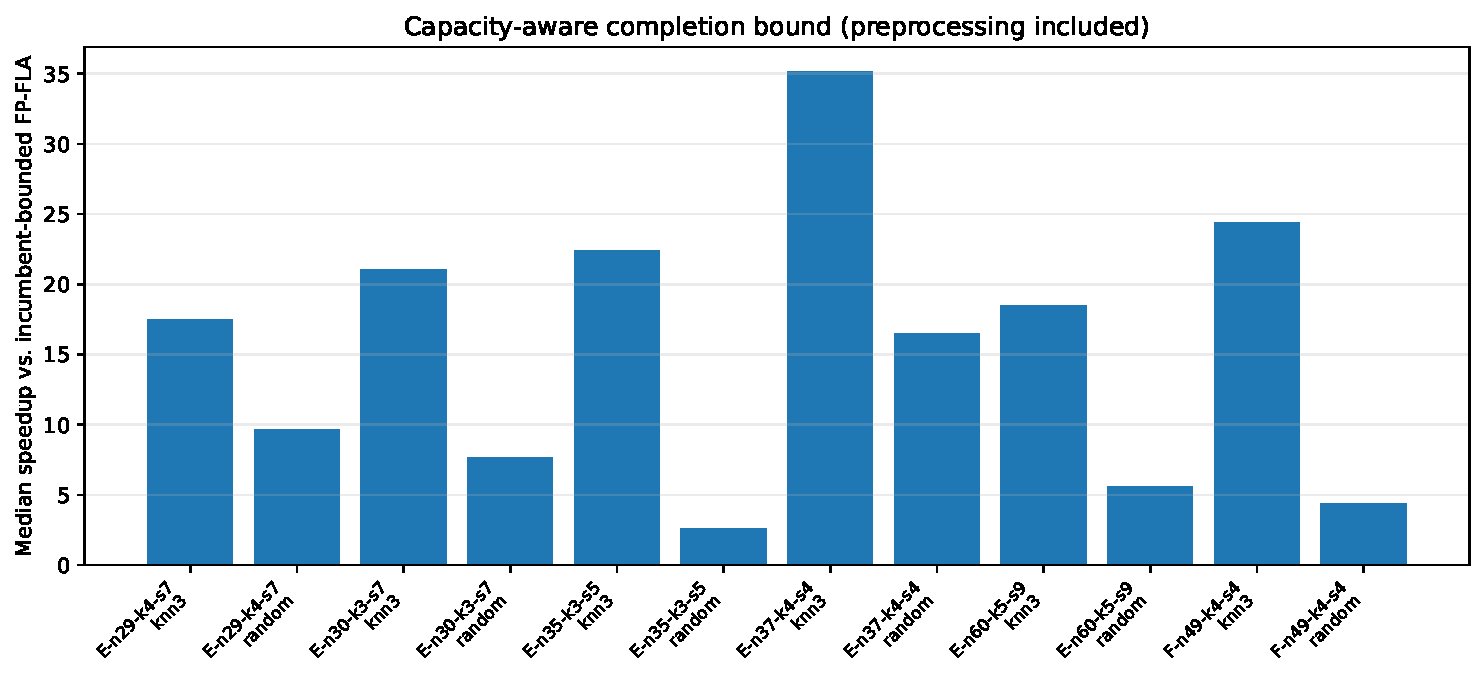
\includegraphics[width=0.94\linewidth]{speedup_by_group.pdf}
\caption{Median preprocessing-inclusive speedup of the capacity-aware decoder relative to incumbent-bounded FP-FLA with the same feasible upper bound.}
\label{fig:speed}
\end{figure}

\begin{figure}[t]
\centering
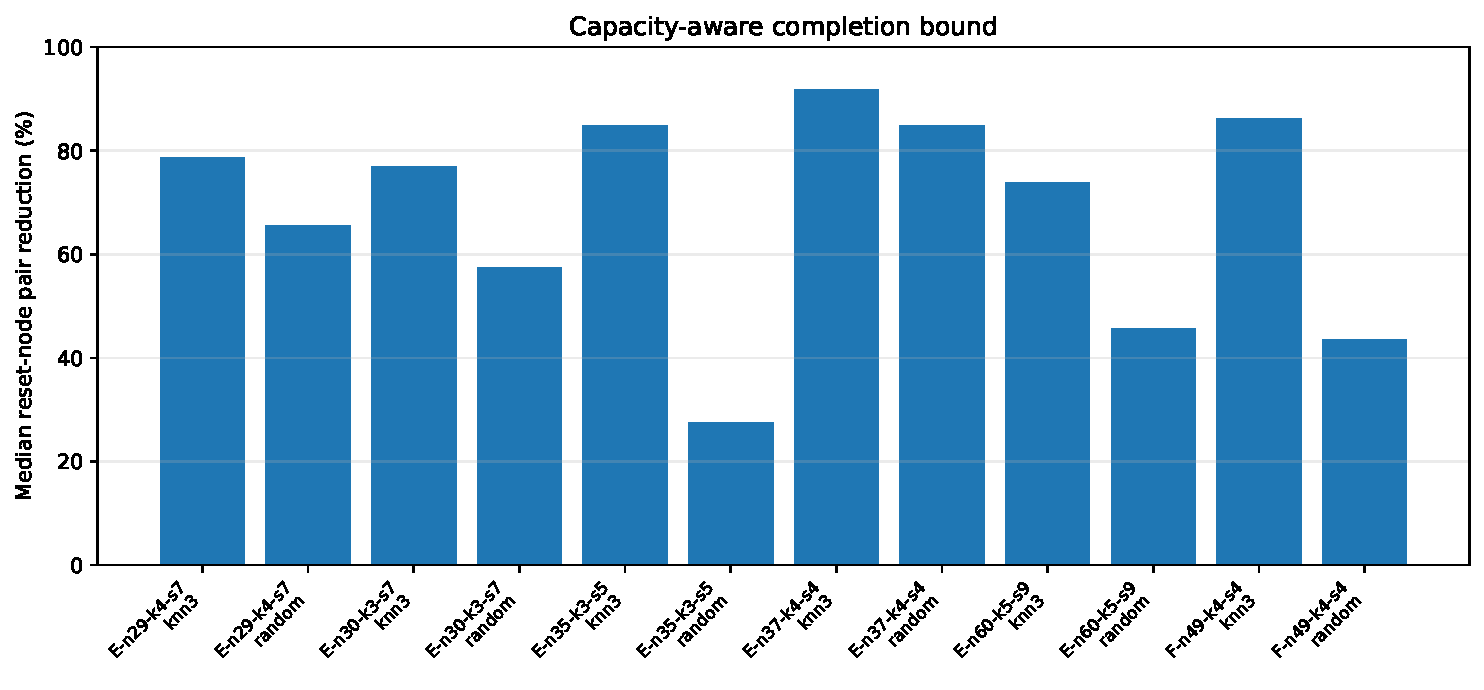
\includegraphics[width=0.94\linewidth]{pair_reduction_by_group.pdf}
\caption{Median reduction in reset-node pair enumeration relative to incumbent-bounded FP-FLA. This count is independent of processor speed and directly measures avoided nested-loop work.}
\label{fig:pairs}
\end{figure}

\FloatBarrier
\subsection{Stress validation}
To test exactness beyond the six public instances, we generated 1,000 synthetic cases across varying customer and station counts using a fixed random seed. Four were infeasible and skipped. On all 996 feasible cases, the incumbent-bounded control, direct lower bound, and capacity-aware bound matched the unbounded source-matched reference objective. The independently constructed initial incumbent was strictly nonoptimal in 425 of those 996 cases. No case required a fallback to an oracle incumbent. The stress output is:
\begin{quote}
\texttt{PASS tested=996 skipped=4 nonopt\_incumbent=425 no\_initial\_incumbent=0}
\end{quote}
This is computational validation rather than a substitute for the proof, but it is useful for detecting implementation errors around equality pruning, capacity endpoints, and dominance interactions.

\subsection{Direct-upstream compatibility gate}
To reduce reliance on the standalone source-matched reimplementation, we also ran a separate gate against the compiled upstream FPSCP core pinned at the following commit:
\begin{quote}\small
\texttt{db9ccca30f2def5fabf85e65958d52dcae0cefd6}
\end{quote}
The gate compares upstream \texttt{OptimalDecode} against a lazy split-DAG construction in which any expensive fixed-block charging subproblem is evaluated by the upstream \texttt{BatteryDecode} itself. Thus both sides exercise the parent project's compiled charging machinery, while the wrapper changes only which block evaluations are requested.

The all-scope gate covered 17 public EVRP instances:
\begin{quote}\small
E-n101-k8, E-n22-k4, E-n23-k3, E-n30-k3, E-n33-k4, E-n51-k5, E-n76-k7, X-n1001-k43, X-n143-k7, X-n214-k11, X-n351-k40, X-n459-k26, X-n573-k30, X-n685-k75, X-n749-k98, X-n819-k171, and X-n916-k207.
\end{quote}
For each instance, 10 uniformly random and 10 nearest-neighbor-biased customer permutations were tested, giving 340 cases. All \textbf{340/340} upstream-vs-lazy objective comparisons matched. One clean-room differential check per instance/permutation family was also retained, giving \textbf{34/34} matches. The hard gate verdict was \texttt{PASS\_EXACT\_REAL\_GATE\_MEASURE\_PERFORMANCE}.

The median fraction of expensive upstream block-oracle calls made by the lazy wrapper was 0.039708 (3.97\%), with mean 0.055441 (5.54\%). The median ratio of wrapper external time to upstream \texttt{OptimalDecode} external time was 0.194738, corresponding to about 5.14x at the median; the mean time ratio was 0.604229. These timings are \emph{auxiliary gate measurements}: the lazy wrapper is not identical to the capacity-aware C++ implementation used for the paper's 14.41x primary benchmark, so the two speedup figures must not be pooled or presented as measurements of the same implementation.

Two wrapper details are important for reproduction. First, the pinned upstream headers use \texttt{std::runtime\_error} without directly including \texttt{<stdexcept>}; on MSVC the comparison wrapper force-included the standard header while leaving the pinned upstream source bytes unchanged. Second, block evaluation uses the partial-route check \path{Solution::is_energy_and_cargo_valid()} rather than the full-instance check \path{Solution::is_valid()}. The latter also requires every customer in the instance to appear exactly once and is therefore inappropriate for a partial depot-to-depot block. An earlier gate run that used full \texttt{is\_valid()} produced 20 systematic mismatches on E-n30-k3; after correcting this wrapper-level validation error, the all-scope gate produced 340/340 matches.

This direct-upstream gate strengthens implementation compatibility evidence, but it is still not an independent external-solver certificate because the comparison deliberately reuses the parent's compiled core.

\section{Discussion}
The principal mechanism is visible in the operation counts: the bound often rejects a label before the $O((|V_f|+1)^2)$ reset-node pair loop. This is qualitatively different from merely checking whether the current partial distance already exceeds $U$. In the public cases, incumbent-only bounding gave only modest runtime change relative to the unbounded reference, whereas the capacity-aware completion term removed a median 73.2\% of reset-node pair enumerations.

The weaker direct-chain bound also helped, but its median speedup versus the same incumbent-bounded control was only 2.94x across the 240 cases. Cargo information therefore supplies most of the additional pruning power. The method is intentionally conservative: it ignores battery constraints rather than attempting to estimate charging cost. This makes admissibility simple and preserves the original state representation. Stronger battery-aware relaxations may provide additional gains, but they must be designed so that any extra state used by the bound does not silently invalidate dominance or exactness.

\paragraph{What is and is not novel.} Completion bounding itself is established in labeling algorithms, including EV routing \cite{froger2019,enerback2024}. We therefore do not claim a new general branch-and-bound principle. The contribution is the specific FPSCP relaxation: retain fixed order and residual cargo capacity, drop battery feasibility, precompute suffix split optima, and use the resulting bound before FP-FLA's station-pair expansion. To the best of our search through September 5, 2026, we found no published follow-up to the May 2026 FPSCP paper that analyzes this specific bound. That literature-status claim should be treated as a scoped search result, not as a proof of priority.

\paragraph{Limitations.} First, the primary 14.41x timing result uses six relatively small benchmark instances and a standalone source-matched reimplementation of the core FP-FLA transitions, not a patch benchmarked inside every metaheuristic from the parent study. The separate 340-case direct-upstream gate materially reduces source-divergence concern for exactness, but its lazy wrapper is a different measurement path and its timing cannot be substituted for the primary capacity-bound benchmark. Neither experiment is an independent MIP/CP certificate. Second, absolute timings in the primary benchmark come from a virtualized Linux environment and are in the microsecond-to-millisecond regime; processor effects can therefore be substantial. Pair counts and front sizes are more robust. Third, the $O(n^2)$ suffix preprocessing is inexpensive for the tested permutations (median 1.57 microseconds) but can matter for much larger $n$. Fourth, the experiments use Euclidean distance and the energy model of the FPSCP parent formulation. Claims should not be transferred without validation to nonlinear charging, time windows, heterogeneous fleets, or nonmetric road costs.

\section{Conclusion}
A fixed customer permutation contains more lower-bound information than FP-FLA's current-distance cutoff uses. By solving a capacity-only suffix relaxation, an exact decoder can quantify the cheapest possible remaining route structure while ignoring battery restrictions. The resulting completion bound is admissible, depends only on the original stage and cargo state, and can be checked before expensive reset-node pair enumeration.

On 240 public benchmark/permutation cases, the proposed capacity-aware variant matched the unbounded source-matched reference objective in every case and achieved a median 14.41x speedup over incumbent-bounded FP-FLA after including bound preprocessing, with a median 73.2\% reduction in reset-node pair enumeration. A further 996 feasible synthetic stress cases produced no mismatch against the same reference construction. Separately, a 17-instance direct-upstream gate produced 340/340 objective matches against the pinned compiled FPSCP core, with 34/34 clean-room checks. The evidence supports using capacity-aware completion bounding as an exact acceleration layer for FPSCP decoding, while leaving the broader choice between exact and restricted decoders to the surrounding metaheuristic and while treating the direct-upstream gate as compatibility evidence rather than an independent solver certificate.

\section*{Artifact Availability}
The accompanying artifact contains the standalone C++ benchmark implementation, stress validator, raw public results, preprocessing measurements, analysis scripts, generated figures, a direct-upstream gate summary, and SHA-256 manifest. The benchmark instance files themselves are not redistributed in the artifact; they are available from the public benchmark repository cited in \cite{mavrovouniotis2020}.

\begin{thebibliography}{9}
\bibitem{uroic2026}
L. S. Uroi\'c and M. \DJ urasevi\'c,
``Where to Split and When to Charge: Optimal Route Construction from Customer Permutations in Electric Vehicle Routing,''
\emph{arXiv preprint arXiv:2605.26816}, 2026. DOI: \href{https://doi.org/10.48550/arXiv.2605.26816}{10.48550/arXiv.2605.26816}.

\bibitem{froger2019}
A. Froger, J. E. Mendoza, O. Jabali, and G. Laporte,
``Improved formulations and algorithmic components for the electric vehicle routing problem with nonlinear charging functions,''
\emph{Computers \& Operations Research}, vol. 104, pp. 256--294, 2019. DOI: \href{https://doi.org/10.1016/j.cor.2018.12.013}{10.1016/j.cor.2018.12.013}.

\bibitem{enerback2024}
J. Enerb\"ack, L. Eveborn, and E. R\"onnberg,
``Pricing for the EVRPTW with Piecewise Linear Charging by a Bounding-Based Labeling Algorithm,''
in \emph{24th Symposium on Algorithmic Approaches for Transportation Modelling, Optimization, and Systems (ATMOS 2024)}, OASIcs 123, pp. 3:1--3:18, 2024. DOI: \href{https://doi.org/10.4230/OASIcs.ATMOS.2024.3}{10.4230/OASIcs.ATMOS.2024.3}.

\bibitem{kullman2021}
N. D. Kullman, A. Froger, J. E. Mendoza, and J. C. Goodson,
``frvcpy: An Open-Source Solver for the Fixed Route Vehicle Charging Problem,''
\emph{INFORMS Journal on Computing}, vol. 33, no. 4, pp. 1277--1283, 2021. DOI: \href{https://doi.org/10.1287/ijoc.2020.1035}{10.1287/ijoc.2020.1035}.

\bibitem{mavrovouniotis2020}
M. Mavrovouniotis, C. Menelaou, S. Timotheou, G. Ellinas, C. Panayiotou, and M. Polycarpou,
``A Benchmark Test Suite for the Electric Capacitated Vehicle Routing Problem,''
\emph{2020 IEEE Congress on Evolutionary Computation (CEC)}, pp. 1--8, 2020. DOI: \href{https://doi.org/10.1109/CEC48606.2020.9185753}{10.1109/CEC48606.2020.9185753}.
\end{thebibliography}

\appendix
\section{Reproducibility Notes}
\small
The public benchmark harness uses deterministic seeds \texttt{20260905} for permutation generation and \texttt{772019} for randomized timing order. The synthetic stress harness uses seed \texttt{917263}. Public runs emit a CSV row only after all exact variants agree with the unbounded source-matched reference. The stress executable exits with a nonzero status on the first mismatch. The main artifact result file contains 240 rows; the stress output records 996 feasible tested cases and four infeasible skips. The direct-upstream all-scope gate contains 340 cases over 17 public instances (10 random plus 10 nearest-neighbor-biased permutations per instance) and records 340 upstream objective matches plus 34 clean-room matches.


\end{document}
